\chapter{Data Analysis}
This chapter is about the analysis of the gathered data. The amplitudes of the signals are recorded and stored. The amplitudes alone say nothing about the signal, except how strong it is. Therefore it is necessary to transform it into the frequency domain via \textit{Fourier Transformation}\footnote{https://betterexplained.com/articles/an-interactive-guide-to-the-fourier-transform/}. This shows which frequencies are involved in the recordings. 
\section{First Prototype}
The first prototype for the detection of clapping was created with Particle's Photon Board. For this purpose the circuit was rebuilt as shown in Figure \ref{fig:photonBoard}\footnote{Source: MSc\_DCSE\_Assignment\_WS6\_Smartphone\_Sensing\_meets\_IoT\_2018\_final} and a test program was loaded with the corresponding Web IDE with which it is possible to collect initial data.
\begin{figure}[h]
	\centering
	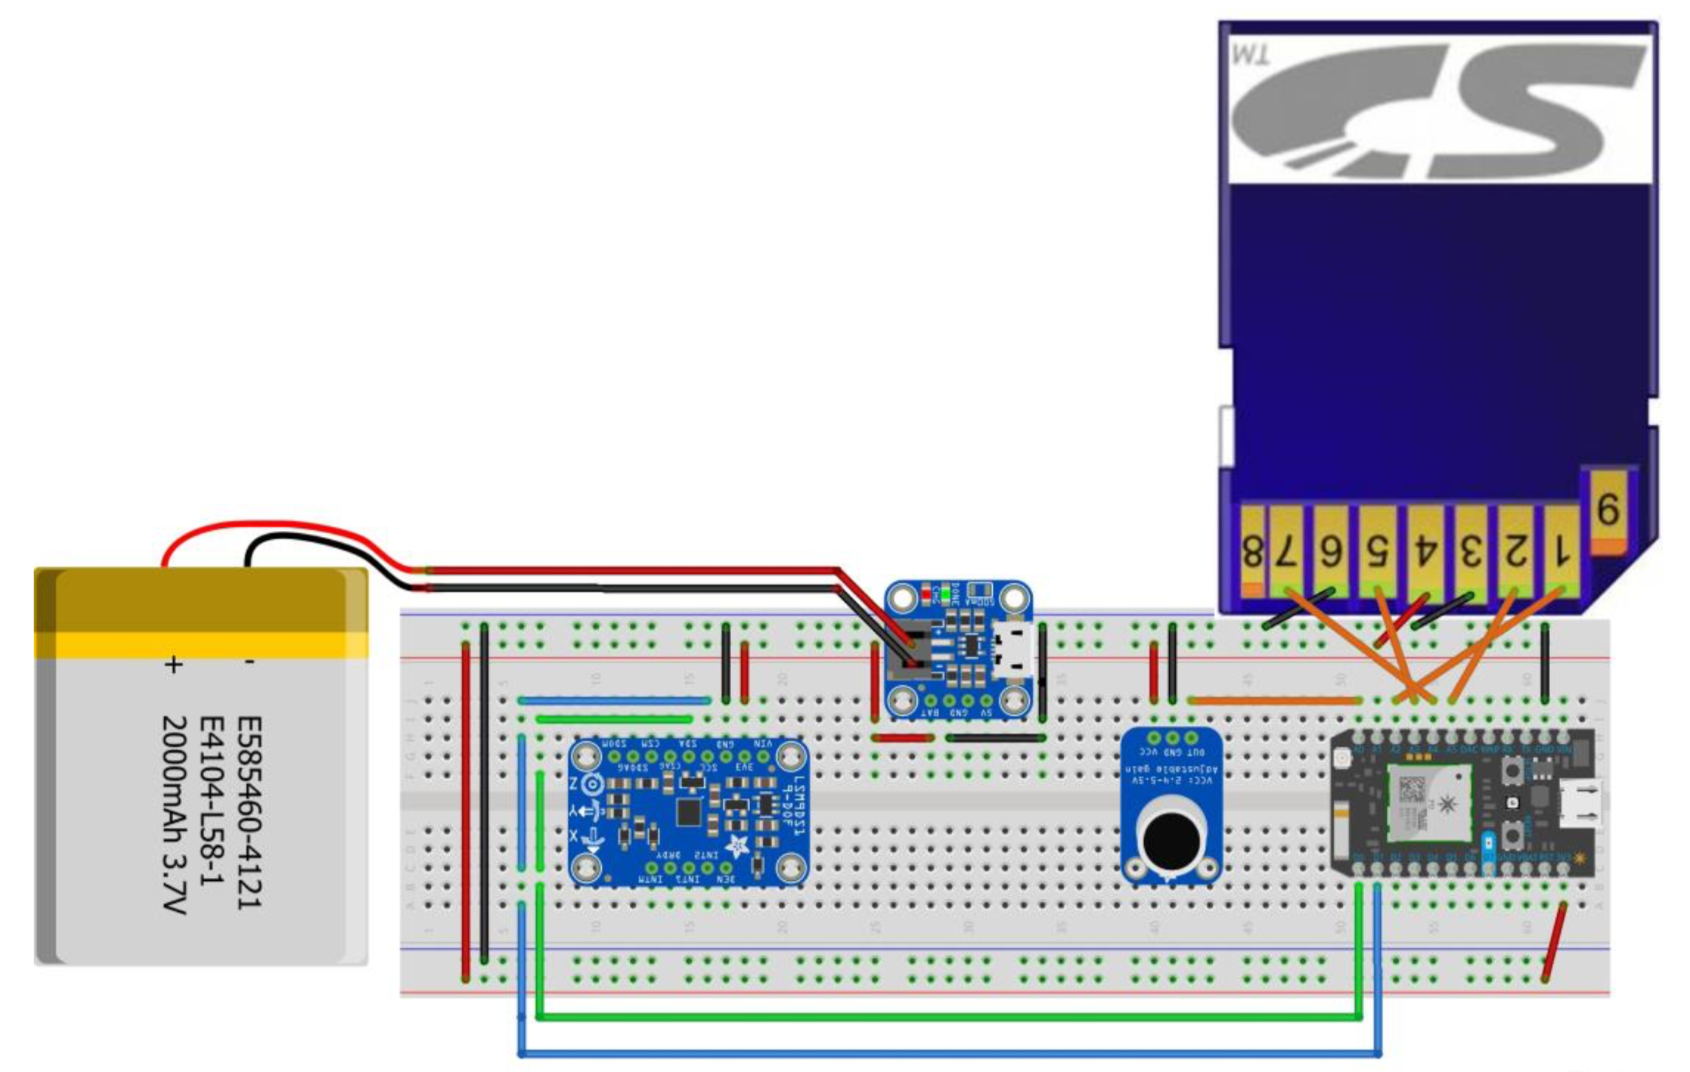
\includegraphics[width=.7\textwidth]{imgs/particleBoard}
	\caption{Particle's Photon Board}
	\label{fig:photonBoard}
\end{figure}
\newpage
The first six measurements were made at a sampling rate of 10Hz. By performing the Fast Fourier transformation on the collected amplitudes, it was possible to examine the amplitude spectrum. Figure \ref{fig:clapping10Hz} shows one result that captured the clapping correctly. This was not the case with every measurement. It can be said that 10Hz is too little for sampling, since possible clapping cannot be measured correctly or only partially in this way. A possible solution is therefore to increase the sampling rate to 1kHz. \newpage
\begin{figure}[h]
	\centering
	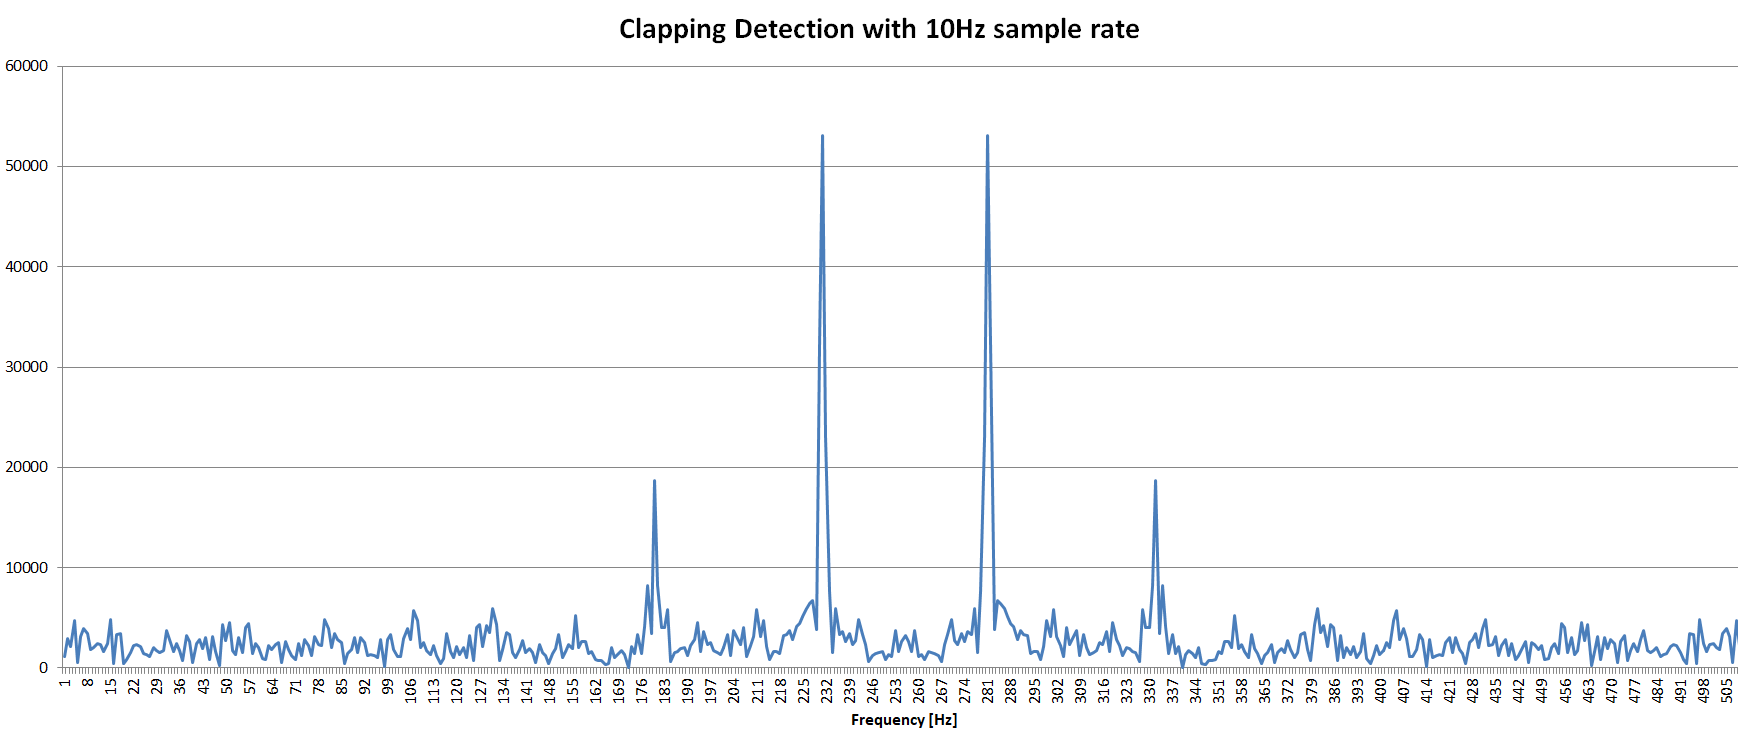
\includegraphics[width=\textwidth]{imgs/clapping10Hz}
	\caption{Amplitude Spectrum for Clapping with 10Hz sample rate}
	\label{fig:clapping10Hz}
\end{figure}
The following measurements have shown that writing to the SD card is too slow in each iteration, resulting in a reduced sampling rate of about 200Hz. It is therefore an idea to keep the data in the memory of the board until enough data has been collected to be written to the SD card at once. 
\\
By holding the data in the memory of the board, it is possible to obtain a higher sampling rate. However, the evaluation of the data is time-consuming, since they first have to be transferred from the SD card to a PC. With many measurements, the time adds up and makes the measurements no longer efficient. \\
Therefore, it makes more sense to use an Android smartphone with its microphone that can send the created CSV files directly, for example to the dropbox. Thus the data is quickly available for several persons and evaluations can be made directly. In addition to that a good debugger, exception handling, as well as reliable and sophisticated libraries for mathematical operations can be used. The implementation of the software for the Android phone and the used libraries are described in more detail in chapter \ref{sec:org11f3563}.
\section{Measurements with Android phone}
According to figure \ref{fig:clappingFreqBereich}\footnote{http://www.klangfuzzis.de/showthread.php?679817-Was-hat-in-etwa-wie-viel-hz} the frequency range of clapping lies between about 120Hz up  to 10kHz. If a 10kHz clapping shall be captured right, the sampling rate according to shannon's law\footnote{http://www.recordingblogs.com/wiki/nyquist-shannon-sampling-theorem} must be double the size of the measured signal. Therefore roughly 20kHz.
\begin{figure}[h]
	\centering
	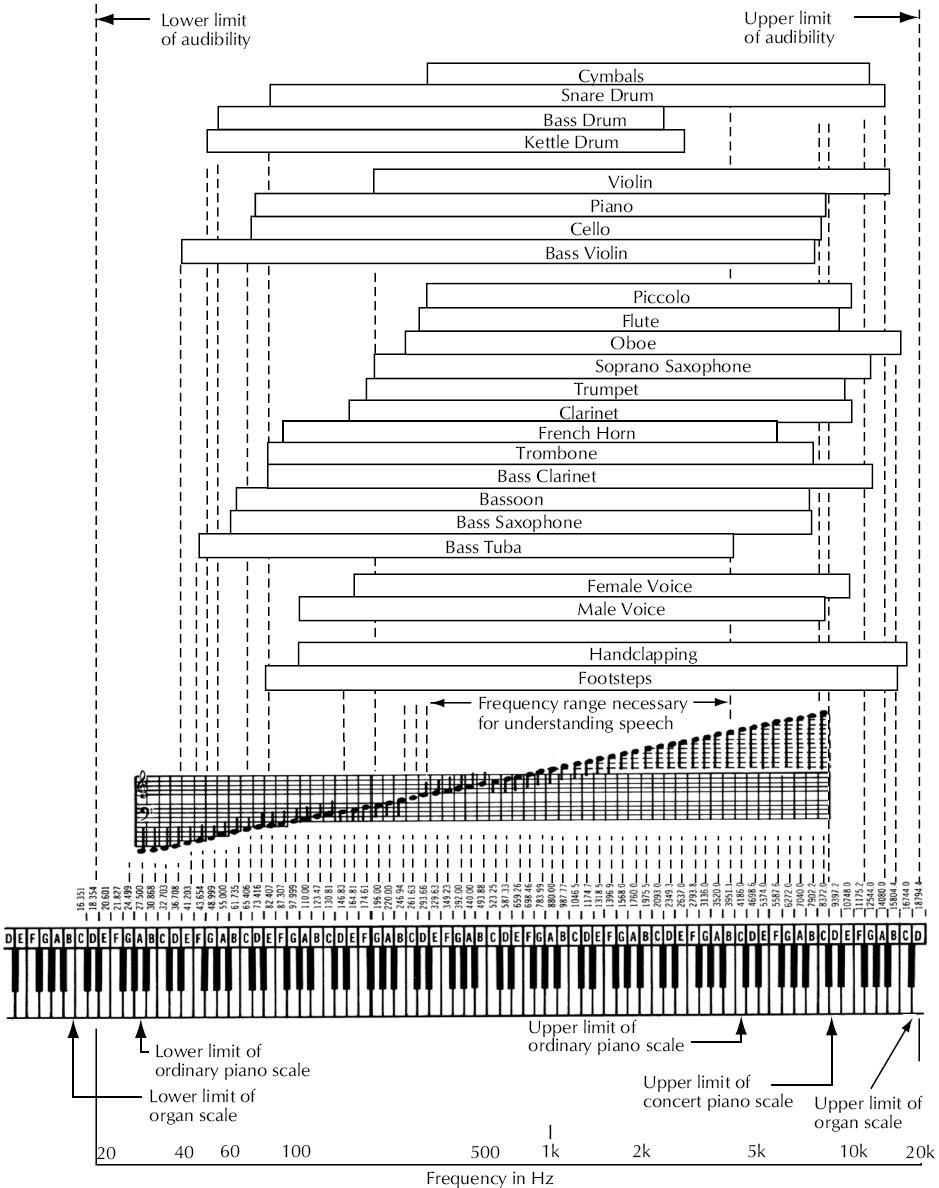
\includegraphics[width=.9\textwidth, trim={0 0 0 5.4cm},clip]{imgs/clappingFreqBereich}
	\caption{Frequency range of clapping}
	\label{fig:clappingFreqBereich}
\end{figure}\\
The first measurements with a sample rate of 22kHz generated the following figure (Figure \ref{fig:clappingAndroid}). Compared to Figure \ref{fig:clapping10Hz}, which shows the signal from the Particle Board, it can be said that the values for the frequency do not match (Table \ref{tab:comparisonParticleAndroid}). This is logical, since the range of the clapping is large. It was tried to perform a nearly similar clapping to retrieve almost identical data. Since this was not the case, an idea was to check the Android Software, if the data was calculated and transformed correctly.\\
\begin{table}[h]
	\centering
	\begin{tabular}{|l|l|}
		\hline
		\textbf{Particle} & \textbf{Android} \\
		\hline
		230Hz & 160Hz\\
		\hline
	\end{tabular}
\caption{Comparison clapping frequency of Particle Board and Android device}
\label{tab:comparisonParticleAndroid}
\end{table}
\begin{figure}[h]
	\centering
	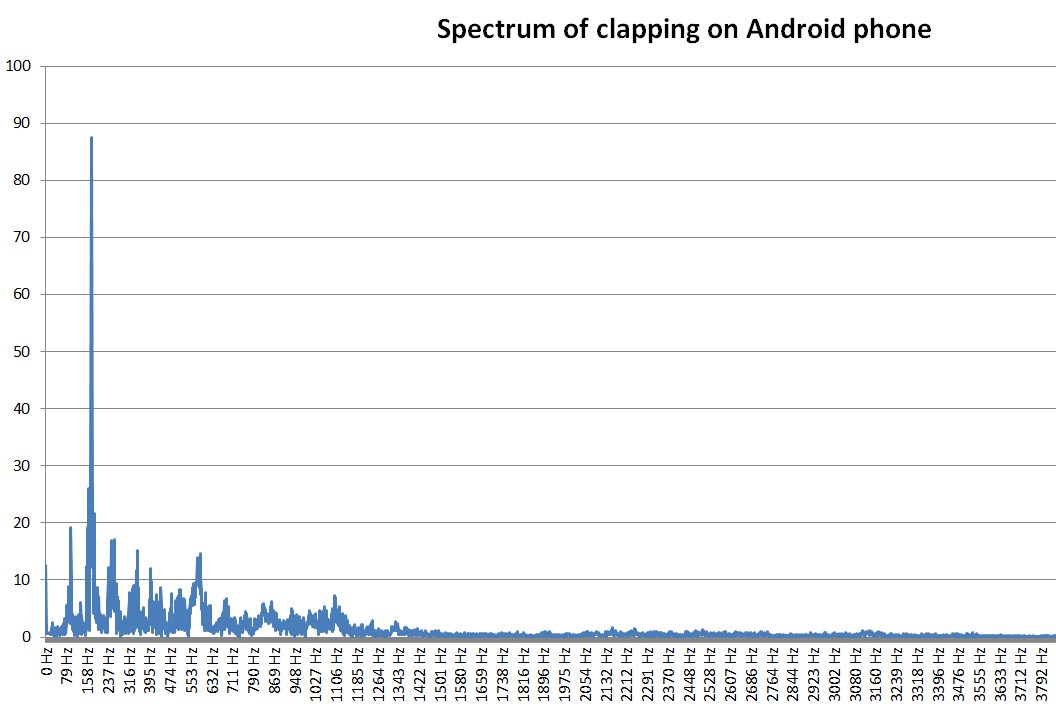
\includegraphics[width=\textwidth]{imgs/clappingAndroid}
	\caption{Amplitude Spectrum for Clapping with Android device}
	\label{fig:clappingAndroid}
\end{figure}\\
For this reason, the check of the calculations is done with another tool called iSpectrum, which can be installed on a MacBook. This makes it possible to collect live data from the laptops microphone to view the spectrum. \\
In order to compare the iSpectrum software and the Android device, a reliable source is needed that provides values for a specific frequency. The idea is to take a sound example and play it to both systems. This makes it possible to observe which values match the frequency.
\\
Instead of a single sound file, a video is used for testing, which plays all frequencies in the audible range of the human ear. This video is called \textbf{20Hz to 20kHz (Human Audio Spectrum)}\footnote{https://www.youtube.com/watch?v=qNf9nzvnd1k} and emits an increasing frequency from 20Hz to 20kHz. It is thus possible to see whether the values are correctly interpreted with different frequencies in the Android device.
\\
As figures \ref{fig:1200HzAndroid} and \ref{fig:1200HziSpectrum} show, the tested frequency of 1200Hz is reliably detected by both systems. Live testing with iSpectrum makes it very convenient to make clapping and other noises visible. Therefore, different sounds were tried out to see what the spectrum looks like.
\begin{figure}[h]
	\centering
	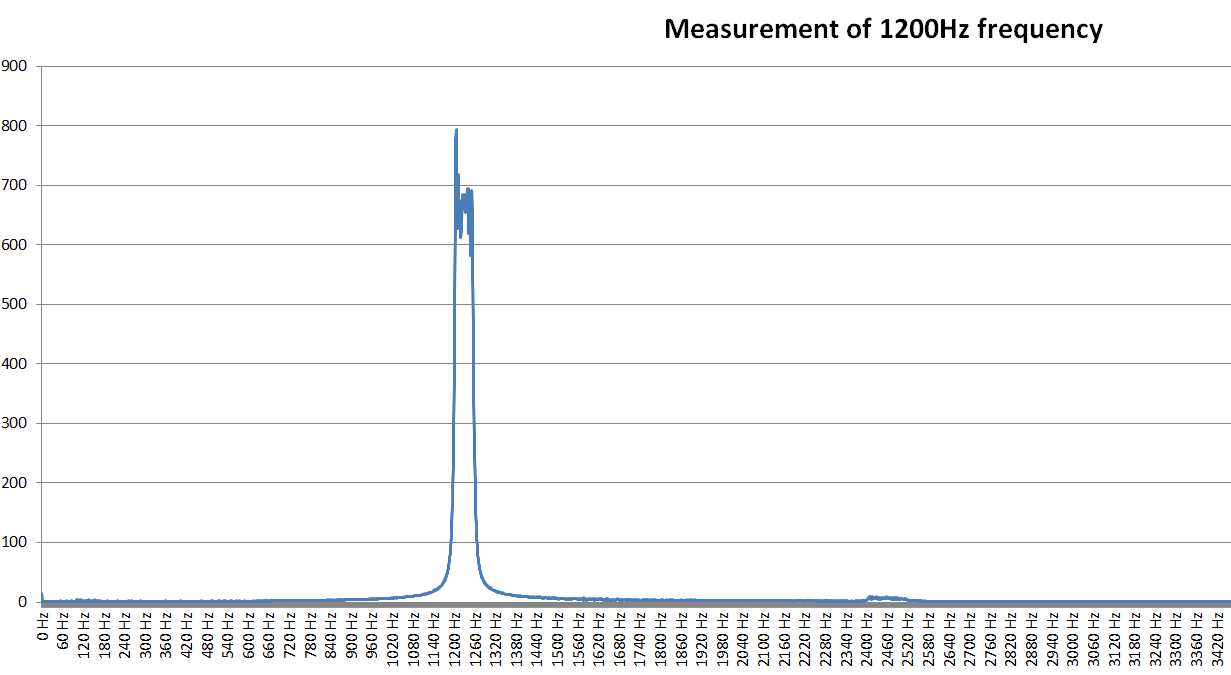
\includegraphics[width=.9\textwidth]{imgs/yt1200Hz}
	\caption{Amplitude Spectrum for 1200Hz (Android device)}
	\label{fig:1200HzAndroid}
\end{figure}
\newpage
\begin{figure}[h]
	\centering
	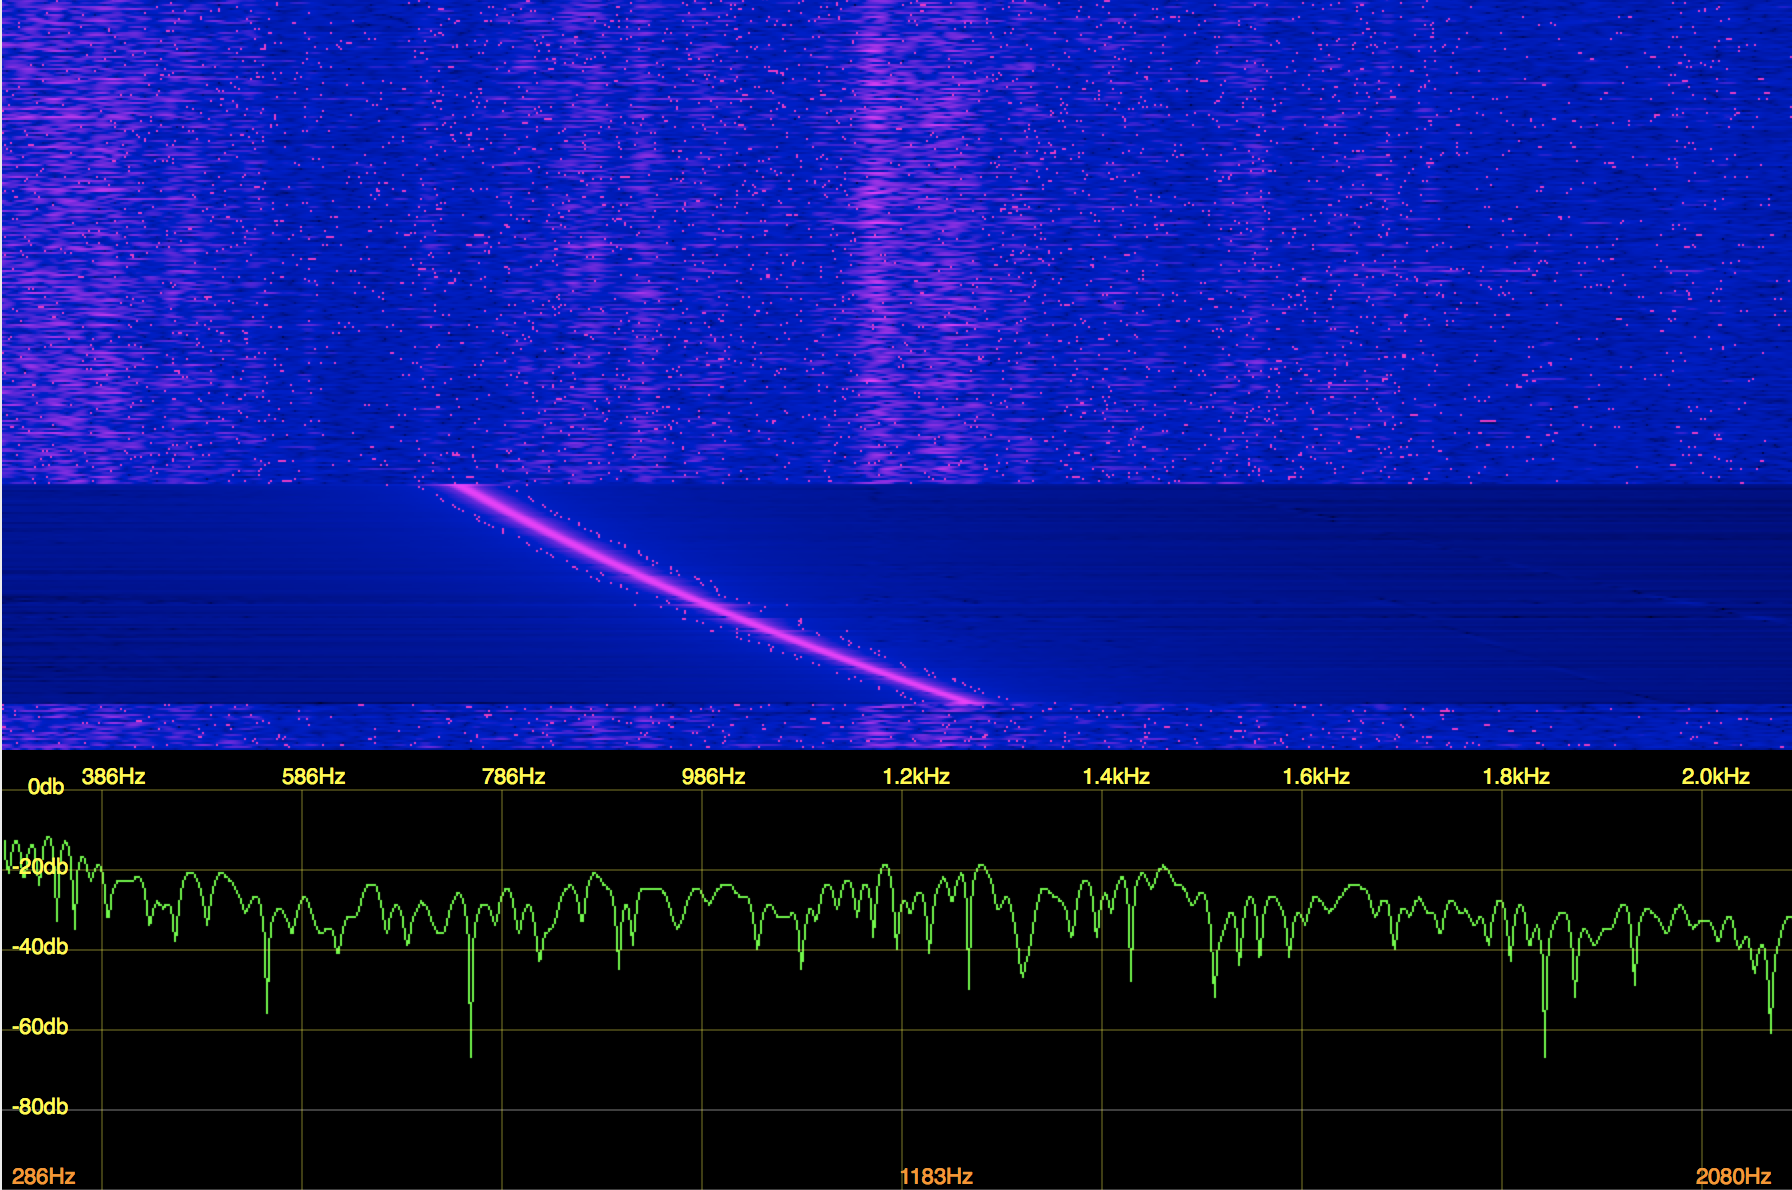
\includegraphics[width=.8\textwidth]{imgs/iSpectrum1200Hz}
	\caption{Amplitude Spectrum from 750Hz to 1200Hz (iSpectrum)}
	\label{fig:1200HziSpectrum}
\end{figure}
The yellow circle in Figure \ref{fig:clappingKnocking} shows the clapping in a small room. The three sounds detected, which have a green frame, are knocking on the table. It can be seen that these noises occur in different frequency ranges. The clapping echoes a little and the knocking stops abruptly. However, each clapping or tapping can be different from person to person, depending on how the clapping or tapping is performed, or where the person is. Further measurements with various test subjects have shown this. Figure \ref{fig:clappingE2} shows clapping from a test person in a big room. It can be obtained, that the clap has more echo in a big room compared to a small room. A distinction between clapping to other sounds could possibly be made with the duration of the echo.
\newpage
\begin{figure}[h]
	\centering
	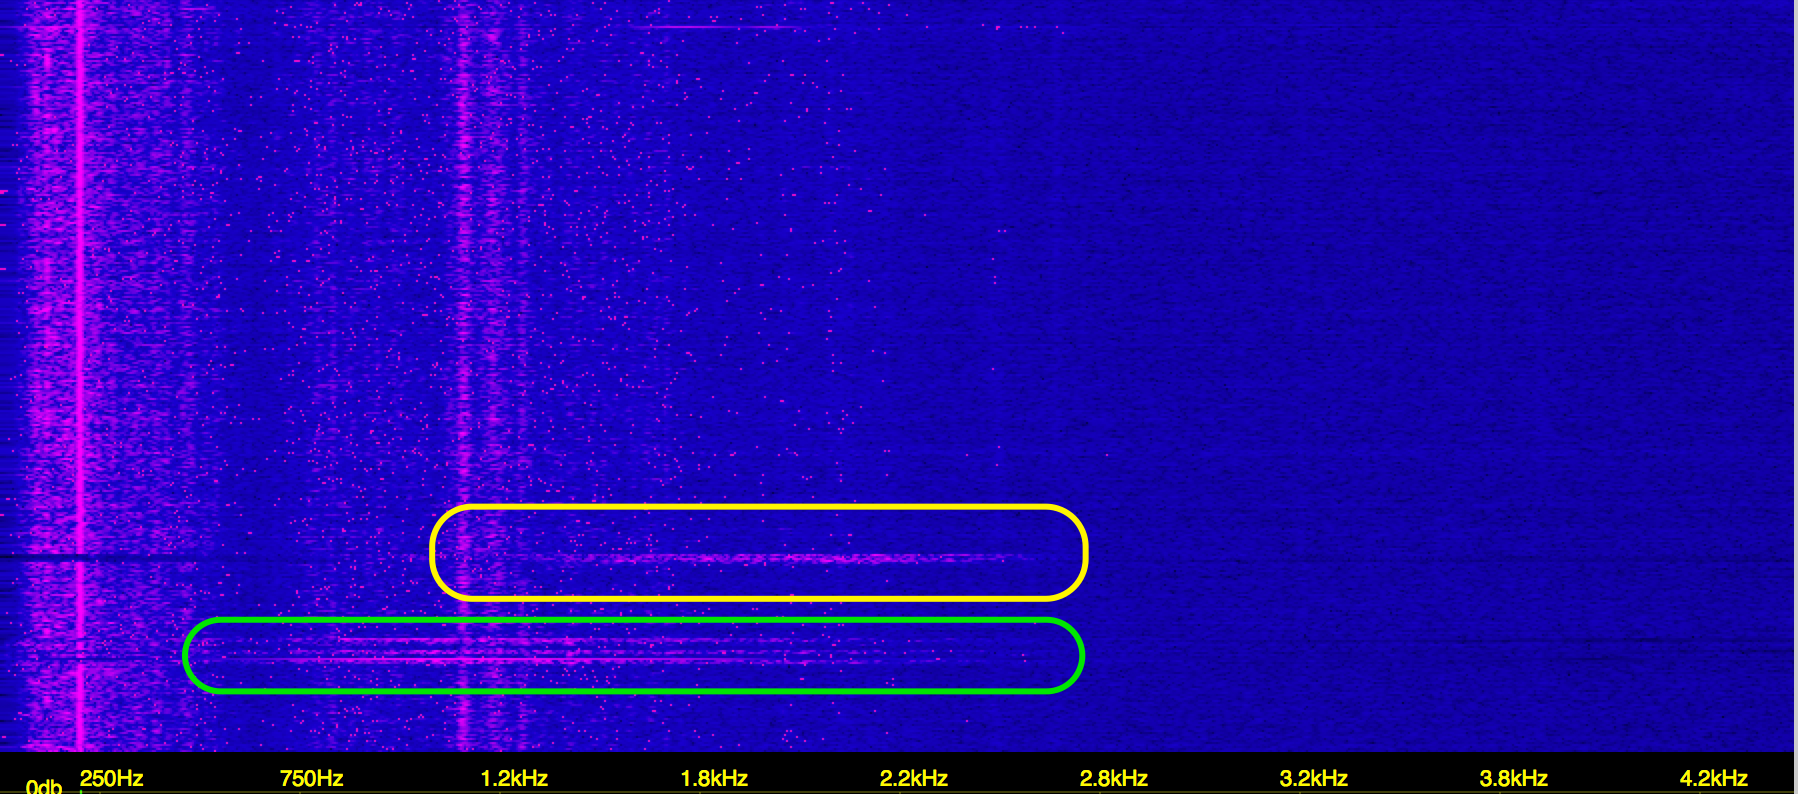
\includegraphics[width=\textwidth, trim={0 0 2cm 5cm},clip]{imgs/iSpectrumClappingKnocking}
	\caption{Spectrum of clapping and knocking}
	\label{fig:clappingKnocking}
\end{figure}
\begin{figure}[h]
	\centering
	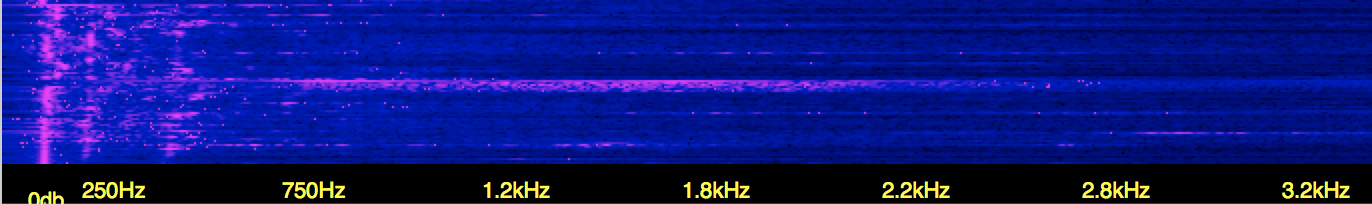
\includegraphics[width=\textwidth]{imgs/iSpectrumClappingE2}
	\caption{Spectrum of clapping in a big room}
	\label{fig:clappingE2}
\end{figure}
\section{Generated insights}
So far, the tests have shown that the clapping is in the range of 750Hz to 3kHz very consistently. That means that the first measurements with 10Hz and 1kHz are not usable, since according to Shannon's law it is not possible to measure this high frequencies with that small sample rate. That is why the first assumptions are completely wrong. Only the measurements with the Android device with a sampling rate of 22kHz provided clearer and more consistent results. Another assumption is that the measurements in Figure \ref{fig:clappingAndroid} give a false impression, since the strongest frequency is in the range around 160Hz. It is possible that the accumulated ambient noise has a higher amplitude than the clapping. This means that the frequency for the clapping is not displayed with a high amplitude. A possible solution for this scenario is to use a digital filter to capture and display only the frequencies of the clapping range. One filter of interest in this case would be the bandpass filter\footnote{https://www.electronics-tutorials.ws/filter/filter\_4.html}, which provides exactly the needed behaviour. The band can therefore be limited from 700Hz to 3kHz.
\\
It is of course very complicated to evaluate every single signal to determine if it is a clap. A single algorithm is therefore not capable of analyzing a wide range of clap frequencies. Therefore it makes sense to evaluate the filtered data with a neural network. However, it should be noted that it takes a lot of training to get a reliable data analysis. This means that many thousands of clap patterns must first be recorded in order to give the neural network the possibility to interpret the clap correctly. TensorFlow\footnote{https://www.tensorflow.org} offers a widely used open source framework for machine learning and provides a good solution strategy for analysing clap signals.